

\section{Miscellaneous}

\subsection{FFT Frequency}

It is surprisingly hard to remember the frequency samples that match the unshifted two-sided discrete Fast Fourier Transform (FFT) for odd or even length signals. Let $f_s$ be the sample frequency and $N$ be the number of points, then the discrete frequencies of the FFT are:

$N$ even:
\begin{equation}
f[k] = \dfrac{f_s}{N}\begin{cases}
    k,& k = 0,..., \dfrac{N}{2} - 1\\
    k-N, & k = \dfrac{N}{2}, ..., N-1 
\end{cases}
\end{equation}

$N$ odd:
\begin{equation}
f[k] = \dfrac{f_s}{N}\begin{cases}
    k,& k = 0,..., \dfrac{N-1}{2} \\
    k-N, & k = \dfrac{N+1}{2}, ..., N-1 
\end{cases}
\end{equation}

The routine \texttt{fftfreq} takes as input the sampling rate, $f_s$, and number of points, $N$, and returns the discrete frequencies $f[k]$ that correspond to the unshifted two-sided FFT of odd or even $N$.

{\footnotesize
\VerbatimInput{\code/Misc/fftfreq.m}
}



\subsection{Phase wrapping}

Phase wrapping is easily done with $\angle \exp(i\phi)$, but there is a fun variation that uses nearest integer rounding written in terms of elementary functions: 
\begin{eqnarray}
\Phi(\phi) & = & \phi - 2\pi\left[\dfrac{\phi}{2\pi} \right] \\
\ & = & -2\arctan\cot\left(\dfrac{\phi}{2} + \dfrac{\pi}{2}\right) 
\end{eqnarray} 

\noindent where $[\cdot ]$ means round to the nearest integer so that $-\pi \le \Phi \le \pi$. %In principle, this can be differentiated away from the wrap points.  

{\footnotesize
\VerbatimInput{\code/Misc/wrap.m}
}

%http://functions.wolfram.com/IntegerFunctions/Round/introductions/FloorRelated/ShowAll.html

%
%\subsection{Complex Standard Normal Distribution}
%
%The complex standard normal distribution is defined
%
%\begin{equation}
%\gamma = \dfrac{1}{\sqrt{2}}\left( \mathcal{N}(0,1) + i \mathcal{N}(0,1)\right)
%\end{equation}
%
%\noindent where $\mathcal{N}(0,1)$ is a normal distribution with zero mean and unit variance.  This is used to add noise to complex signals or to seed power spectral densities (PSD) in the frequency domain. For the later, we require $\gamma$ to have conjugate symmetry if the inverse Fourier transform is to yield a real valued signal. Because the Fourier transform of a Gaussian random variable is also Gaussian, a lazy way to ensure conjugate symmetry is to take the DFT of an array loaded with the real valued standard normal. However, a faster and more practical way to generate a signal from a PSD is simply to seed the PSD with the complex standard normal, without conjugate symmetry, and take the real part after the IFFT.  
%
%The routines \texttt{gamman} and \texttt{gammanw} return the complex standard normal and frequency domain complex standard normal, respectively, for an arbitrary number of dimensions of sizes $N_1$, $N_2$, etc.  The frequency domain version is computed with the DFT, which requires division by the dimension lengths.  It can be verified that for both the real and imaginary parts of each functions that the mean and variance are $0$ and $1/\sqrt{2}$, respectively.  In \texttt{gammanw}, we set the DC component to zero to guarantee zero mean.  
%
%{\footnotesize
%\VerbatimInput{\code/Misc/gamman.m}
%}
%
%{\footnotesize
%\VerbatimInput{\code/Misc/gammanw.m}
%}

\clearpage
\newpage
\subsection{Cubic Roots}

The roots of a cubic polynomial are known analytically. Let the cubic be written
\eq{a x^3 + b x^2 + c x + d = 0}

and define
\ea{w &=& -\dfrac{b}{3a} \\
Q &=& \dfrac{3ac - b^2}{9a^2} \\
R&=& \dfrac{9abc - 27a^2d - 2b^3}{54a^3} \\
D &=& Q^3 + R^2}

When $D\ge0$, there is one real root and two complex conjugate roots. For this case, define
\ea{S &=& \sqrt[3]{R + \sqrt{D}} \\
T &=&  \sqrt[3]{R - \sqrt{D}} }

When $D < 0$, there are three real roots and the following is used
\ea{S &=& \sqrt[3]{\rho}e^{i \theta/3} \\
T &=&  \sqrt[3]{\rho}e^{-i \theta/3} \\
\rho &=& \sqrt{-Q^3} \\
\theta &=& \arccos\left(\dfrac{R}{\rho}\right)}

In all instances, the positive roots of $\sqrt[3]{}$ and $\sqrt{}$ are used. The roots of the cubic are then given by 
\ea{x_1 &=& w + S + T \\
x_2 &=& w -\dfrac{1}{2}(S +T) + i\dfrac{\sqrt{3}}{2}(S-T) \\
x_3 &=& w -\dfrac{1}{2}(S +T) - i\dfrac{\sqrt{3}}{2}(S-T) }

\noindent where $x_1$ is always real.

The routine \texttt{cubicroots} is a vectorized implementation of the solution above that computes the roots of multiple cubic polynomials simultaneously. Coefficient arrays can be any size. When \texttt{nargout == 1}, the routine returns the guaranteed real root $x_1$. The key difference between this routine and Matlab's \texttt{roots} is that \texttt{roots} is not vectorized and only solves one polynomial at a time, otherwise, the two routines produce the same solutions.

{\footnotesize
\VerbatimInput{\code/Misc/cubicroots.m}
}

\subsection{Quartic Roots}

Like the cubic, the roots of a quartic polynomial are known analytically, \cite{weisstein_quartic}.  Let the quartic be written 
\eq{a x^4 + b x^3 + c x^2 + d x + e = 0}

This is put in standard form by dividing the leading coefficient
\eq{x^4 + a_3 x^3 + a_2 x^2 + a_1 x + a_0 = 0}

\noindent where $a_3 = b/a$, $a_2 = c/a$, $a_1 = d/a$ and $a_0 = e/a$.  This has resolvent cubic
\eq{y^3 - a_2y^2 + (a_1a_3-4a_0) y + (4 a_2 a_0 - a_1^2-a_3^2 a_0) = 0 \label{resolvecube}}

If $y_1$ is any real root of \eqref{resolvecube} (there is always at least one), then the roots of the quartic are given by 
\ea{x_{1,2} &=& w + \dfrac{1}{2}R \pm \dfrac{1}{2}D \\
x_{3,4} &=& w - \dfrac{1}{2}R \pm \dfrac{1}{2}E }

\noindent where
\ea{ D &=& \begin{cases}  \sqrt{T - R^2 + \dfrac{U}{R}}, \quad R\ne 0 \\ \sqrt{T + V},\quad \quad \quad \quad R = 0 \end{cases} \\
E &=& \begin{cases}  \sqrt{T - R^2 - \dfrac{U}{R}}, \quad R\ne 0 \\ \sqrt{T - V}, \quad \quad \quad \quad R = 0 \end{cases} }

and
\ea{w &=& -\dfrac{1}{4} a_3 \\
R &=& \sqrt{\dfrac{a_3^2}{4} - a_2 + y_1} \\
T &=& \dfrac{3 a_3^2}{4} - 2 a_2\\
U &=& \dfrac{4a_3a_2-8a_1-a_3^3}{4} \\
V &=& 2 \sqrt{y_1^2 - 4 a_0} }


The routine \texttt{quarticroots} is a vectorized implementation of the solution above that computes the roots of multiple quartic polynomials simultaneously. Coefficient arrays can be any size. The real cubic root, $y_1$, comes from \texttt{cubicroots}. Again, Matlab's \texttt{roots} only solves one polynomial at a time, otherwise the two routines produce the same solutions.

{\footnotesize
\VerbatimInput{\code/Misc/quarticroots.m}
}

\clearpage
\newpage
\subsection{Uniform Points on a Sphere}

A quick approximation of uniform points on a sphere is based on the disco ball. Points are distributed mostly evenly at discrete latitudes centered on a prime meridian. This avoids crowding at the poles that happens with uniform sampling in spherical coordinates. Specifically, the number of lines of latitude is chosen which are divided equally between $\theta = [0, \pi]$, then each circle of constant latitude is divided by the latitude spacing as many times as it will go.

The routine \texttt{discoball} takes as input the number of latitude lines \texttt{nlat} and returns the spherical coordinates of the points $(\theta,\phi)$.  

\begin{figure}[H]
\centering
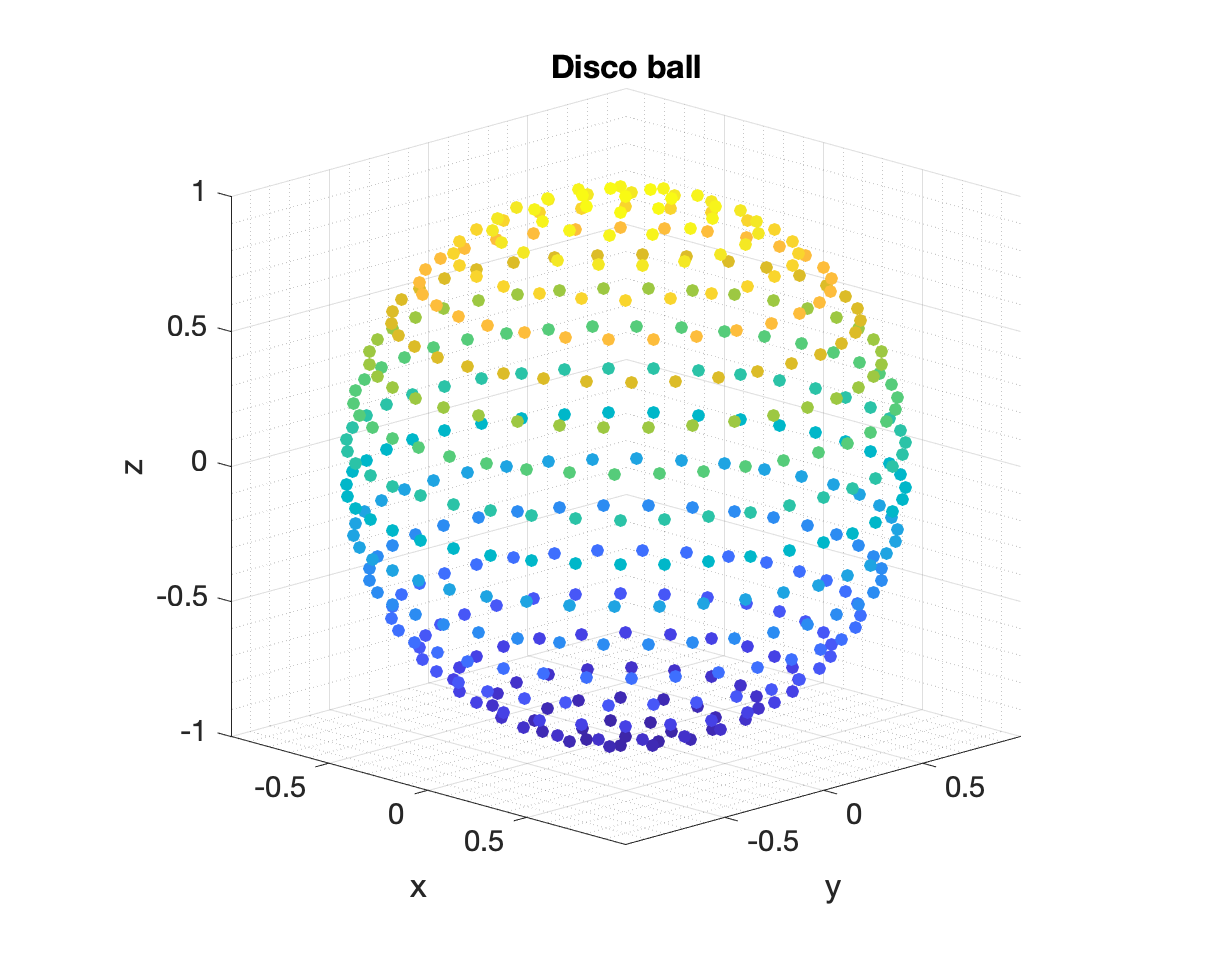
\includegraphics[width=3.5in]{Utilities/Figures/discoball}
\caption{Disco ball approximation for uniform points on a sphere}
\end{figure}

{\footnotesize
\VerbatimInput{\code/Misc/discoball.m}
}

\clearpage
\newpage

\subsection{Uniformly Random Points on a Sphere}

To create a set of points that are uniformly random over the unit sphere, it is not correct to draw from a uniformly random distribution of spherical angles $(\theta,\phi)$, because this leads to crowding at the poles.  Instead, the following transformation is used, \cite{randsphere}, 
\begin{eqnarray}
\phi &=& 2\pi U(0,1) \\
\theta &=& \arccos(2V(0,1)-1)
\end{eqnarray}

\noindent where $U(0,1)$ and $V(0,1)$ are uniform random variables from $[0,1]$.  

The routine \texttt{randsphere} takes as input the total number of points, $N$, and returns the spherical $(\theta,\phi)$ coordinates of the points.  

\begin{figure}[H]
\centering
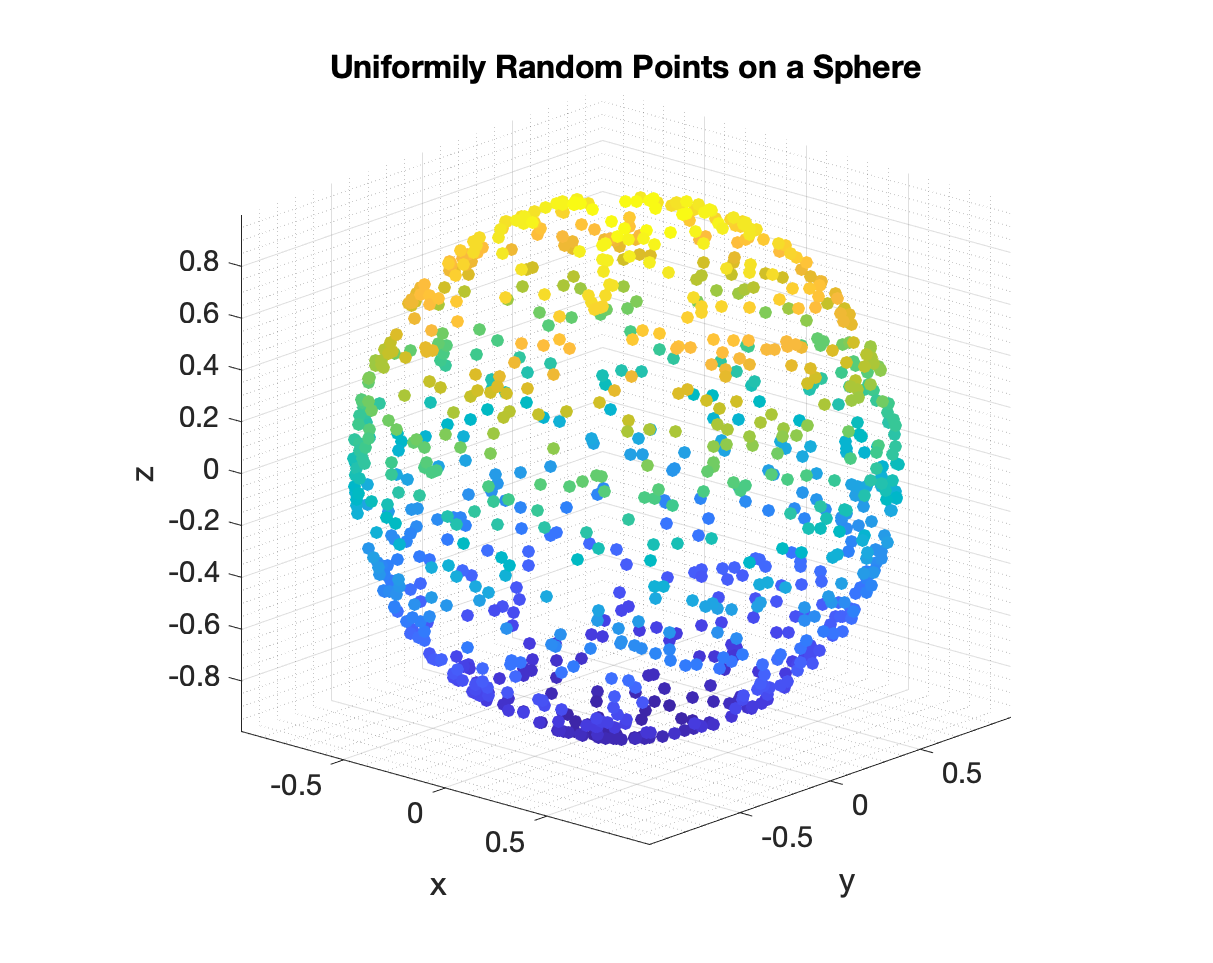
\includegraphics[width=3.5in]{Utilities/Figures/uniformrand}
\caption{Uniformly random points on a sphere, $N = 1000$. }
\end{figure}

{\footnotesize
\VerbatimInput{\code/Misc/randsphere.m}
}

%
%\subsection{$\log_b(x)$}
%
%Matlab doesn't have this.
%
%\begin{equation}
%\log_b(x) = \log(x)/\log(b)
%\end{equation}
%
%{\footnotesize
%\VerbatimInput{\code/Misc/logb.m}
%}
%
%\subsection{Triangle Function}
%
%The standard triangle function is given by
%
%\begin{align}
%\textrm{tri}(t) = 
%& = \max(1 - |t|, 0) \\
%&= 
%\begin{cases}
%1 - |t|, & |t| < 1 \\
%0, & \mbox{otherwise} 
%\end{cases}
%\end{align}
%
%This can be generalized to a triangle with arbitrary width, height, horizontal and vertical offsets as
%
%\begin{equation}
%\textrm{tri}(t) = \max\left(b\left(1-\left\vert \dfrac{x-x_o}{a} \right\vert \right) + y_o, y_o\right)
%\end{equation}

%
%{\footnotesize
%\VerbatimInput{\code/Misc/triangle.m}
%}

